\chapter{Selection Bias Removal}
\label{ch-sb-removal}
This chapter
is based on Ref.\cite{bare-sb-removal}.

Selection bias (SB)
occurs when one
samples from an
atypical subset
of a
population,
producing a biased dataset.
Are such biased
datasets
useless? Not necessarily.
It is possible to
add auxiliary features
to the biased dataset, and to
sample those new features
in an unbiased way,
 from the whole population.
Then
one can merge
the original
 biased dataset with the
auxiliary, unbiased one,
to obtain an enhanced dataset.
It is sometimes
possible to do this so that the enhanced
dataset is provably
unbiased.
It's like making horizontal
the surface of a table
 that was
 not initially
horizontal.
The theory of Bayesian Networks and Causal
Inference tells us
WHEN this is possible,
and HOW to do it
when it is possible.

Consider the bnet
Fig.\ref{fig-bs-removal-basic}.

\begin{figure}[h!]
$$
\xymatrix{
\rvs=1
&*+[F]{\rvA}\ar@{<->}[d]\ar[l]_?
&
\\
\rvx\ar[r]\ar[u]_?\ar@/_.9pc/@{<->}[ru]
&\rvy\ar[ul]_?
}
$$
\caption{Bnet considered for
selection bias (SB) removal.
Arrows with question marks
may or may not be present.}
\label{fig-bs-removal-basic}
\end{figure}

Let

$\rvs\in\bool$
be the {\bf selection node}.
$\rvs=1$ means there is
SB
in the parent nodes.


$\rvx=$ {\bf class features}.\footnote{
A feature is the same as a node in a bnet.}

$\rvy=$ {\bf target feature}.

$\rvA=$ {\bf auxiliary features}.
This is a set of nodes that
may contain arrows entering
or exiting it, as indicated by the double arrows.

$\rvE=\{\rvy, \rvx\}\cup\rvA=$
{\bf Enhanced feature set}.


$\Sigma=$ unbiased population of individuals $\s$

$\Sigma_o=$ biased sub-population of individuals,
$\Sigma_o\subset \Sigma$.

$OD=\{({\s_o},\rvx^{\s_o},  \rvy^{\s_o},\rvs^{\s_o}=1):{\s_o}\in\Sigma_o\}=$
{\bf Original Dataset}, dataset for $(\rvx,\rvy)$ features
with $\rvs=1$.
Gives empirical
distribution $\color{red}{P(y|x, \rvs=1)}$.
(Ref.\cite{bare-sb-removal}
calls this dataset the {\bf biased study}.)

$AD=\{(\s, \rvx^\s,\rvA^\s):\s\in\Sigma\}=$
{\bf Auxiliary Dataset}, dataset for $(\rvx, \rvA)$ features.
Gives empirical
distribution $\color{red}{P(A|x)}$.
(Ref.\cite{bare-sb-removal}
calls this dataset the
{\bf population level study}.)


$ED=\{({\s_o},\rvx^{\s_o}, \rvA^{\s_o}, \rvy^{\s_o},
\rvs^{\s_o}=1):{\s_o}\in\Sigma_o\}=$
{\bf Enhanced Dataset}, dataset for $(\rvx,\rvy, \rvA)$ features
for $\rvs=1$.
Obtained by merging $OD$ and $AD$.
Gives empirical
distribution $\color{red}{P(y|x, A, \rvs=1)}$.

\section{Pre and Post Selection Nodes}
Selection
nodes can be a source
of confusion,
so it's worth
spending some time
thinking about them.

This book uses 2 types of selection nodes:
pre-selection nodes and post-selection nodes.

{\bf pre-selection nodes} are used
in Chapter \ref{ch-transport}
entitled ``Transportability
of Causal Knowledge".
Suppose that the nodes
of a bnet can be either
blue or colorless.
Then we can define
a pre-selection
node $\rvs_{blue}$
such that
$\rvs_{blue}=1$
points
to the nodes that
are blue, and
nothing
points
to the nodes that are
colorless.
If we were to
change the value of
node $\rvs_{blue}$ to
zero,
then all the nodes
of the bnet would be colorless.
Suppose instead that
the nodes of a bnet
could be either
blue, red or colorless.
Then one could define
two pre-selection nodes,
$\rvs_{blue}$
and $\rvs_{red}$,
and
draw arrows
from $\rvs_{blue}=1$
to the blue nodes
and from
$\rvs_{red}=1$
to the red nodes, and no arrow
directed into the colorless nodes.
So, basically, pre-selection nodes
are binary {\color{red}root} nodes
that indicate
whether the nodes pointed to
belong to a set or not.

Most of the DAG literature,
including Ref.\cite{bare-sb-removal},
on which this chapter is based,
define SB using a {\bf post-selection node}.
A post-selection node
is a binary {\color {red}leaf} node
of the graph.

\begin{figure}[h!]
\centering
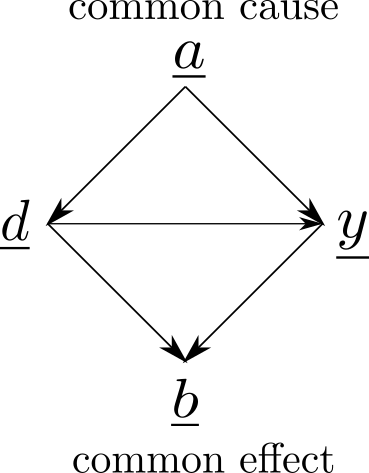
\includegraphics[width=1in]
{sb-removal/common-cause-effect.png}
\caption{Common Cause
and Effect for
nodes $\rvd,\rvy$.}
\label{fig-common-cause-effect}
\end{figure}

Note
that in Potential
Outcomes (PO) theory
 (see Chapter \ref{ch-pot-out}),
pre-selection nodes such
as $\rva$ in
Fig.\ref{fig-common-cause-effect}
are called {\bf common cause
 (confounder, fork) nodes
for nodes $\rvd, \rvy$}.
Furthermore, post-selection nodes such as
$\rvb$ in
Fig.\ref{fig-common-cause-effect} are
called
{\bf common effect
(selection bias (SB), collider) nodes
for nodes $\rvd, \rvy$}.
Hence, in PO theory,
SB is indicated
by
a leaf node,
just as we do in this chapter.

Note that
{\bf Simpson's paradox} (see Chapter
\ref{ch-simpson}) arises from an indirect effect
caused by \ul{not conditioning}
on a confounder,
whereas
{\bf Berkson's paradox}
(see Chapter \ref{ch-berkson})
arises from an indirect effect
caused by \ul{conditioning}
on a collider.



It's possible to replace a pre-selection node
by a post selection node, or vice versa, as
follows.
Suppose that we start with
a bnet $G_0$ that is fully connected, and
we add to it a selection node $\rvs$
that is a root node that points
to all nodes of $G_0$.
Call the resulting bnet $\rvs\rarrow G_0$.
We can use Bayes rule to reverse the direction
of the arrows emanating from $\rvs$
so that they enter node $\rvs$
rather than exit
it.
Call the resulting bnet $\rvs\larrow G_0$.
In general,
Bayes rule allows us to translate
from $\rvs\rarrow G_0$ to
$\rvs\larrow G_0$,
or in the opposite direction,
without having to change the
directions of any of the arrows in $G_0$.
If $G_0$ is not fully connected, then
going from
$\rvs\rarrow G_0$ to
$\rvs\larrow G_0'$
will often require that $G_0'$
have the same arrows in the same
directions as $G_0$
plus some extra arrows
new to $G_0$.
Likewise, going
from
$\rvs\larrow G_0$ to
$\rvs\rarrow G_0''$
may require that $G_0''$ have
the same arrows as $G_0$ plus some new arrows.

So far, we have
been intentionally
vague in specifying the graphs
$G_0'$ and $G_0''$.
In Fig.\ref{fig-sel-nd-reversal}
we give a trick for determining
possible candidates for
graphs $G_0'$ and $G_0''$.
In
Fig.\ref{fig-sel-nd-reversal},
we consider 3 panels going from left
to right, depicting
the cases where $\rvs$ has either 1,2 or 3 neighbors.
The top graph
 $G_{post-sel}$, which has
a post-selection node $\rvs$, is converted
to a graph which is numerically
equal to it, namely
the bottom
graph
 $G_{pre-sel}$, which has
a pre-selection node $\rvs$.
The magenta arrows represent
any number of arrows
exiting (but none entering)
a node.
If we start
with a graph $s\larrow G_0$,
we find the biggest subset $X$ of
the nodes of $G_0$ such
that $\rvs\larrow X$ only has nodes
exiting it (i.e., only magenta nodes).
Then we add enough
arrows to $\rvs\larrow X$
to make it a fully connected graph
$\rvs\larrow X'$.
Now we can reverse the incoming
arrows to $\rvs$ and make them
all outgoing and call the
resulting graph $\rvs\rarrow X'$.


\begin{figure}[h!]
\centering
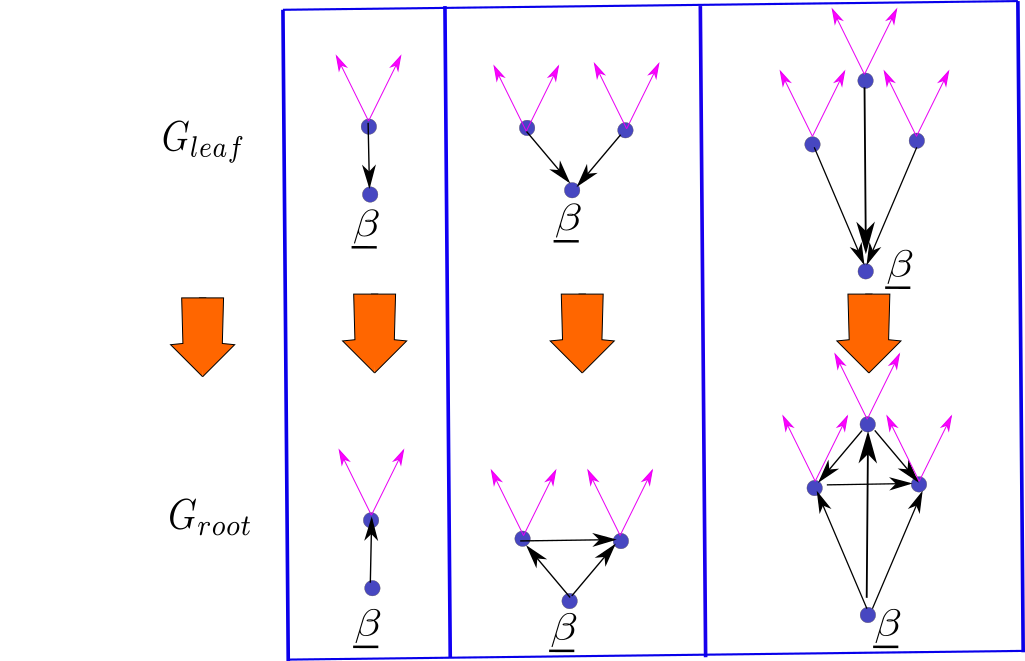
\includegraphics[width=4in]
{sb-removal/sel-nd-reversal.png}
\caption{Switching
from a post-selection node
to a pre-selection node.}
\label{fig-sel-nd-reversal}
\end{figure}

Recall that in Chapter [\nameref{ch0-bnet-def}],
we made a distinction
between a good CF bnet
a bad CF bnet, and
we pointed out
that bad CF bnets are
often useful as
a numerical tool.
Recall also from Chapter
\ref{ch-obs-equi}
that two bnets can be
``observationally equivalent".
That is what is happening here.
We are faced with
the choice of
making selection nodes
either
leaf nodes or root nodes.
Both
choices  lead to observationally
equivalent bnets.
One of the two choices
leads to a good
CF bnet,
and the other to a bad CF bnet.
Both choices are numerically
correct.

In this
chapter,
we will consider
first a DAG $G_{post-sel}$ with a post-selection
node, then we will transform that
DAG to a numerically equal
DAG $G_{pre-sel}$
with a pre-selection node.
The latter DAG
is more convenient
for our needs. Why?
Because
in the SB theory
that we present in this chapter, the
$\rvs=1$
appears as a condition in a conditional
probability,
as in $P(\cdots|\cdots, \rvs=1)$.
Such probabilities
are represented  in a more
straightforward manner if arrows
exit rather than enter node
$\rvs$.




\section{Removing SB from
passive query $P(y|x)$}

The {\bf  passive query} $Q=P(y|x, \rvs=1)$
is {\bf SB-recoverable}
if it is independent of $\rvs$.







\begin{enumerate}
\item
{\bf Query $P(y|x)$ is
SB-recoverable}
with $\rvA= \emptyset$; SB can be removed
by conditioning on $\rvx$.

If $\rvy\perp\rvs|\rvx$, then
\beq
P(y|x, \rvs=1)=P(y|x)
\;.
\eeq
For example,

\begin{subequations}
\label{eq-recoverable-null-A}
\beq
\begin{array}{ccc}
\xymatrix{
\rvs
\\
*++[o][F*:yellow]{\rvx}\ar[u]\ar[r]&\rvy
}
&
\xymatrix{\\=}
&
\xymatrix{
\rvs\ar[d]
\\
{\rvx}\ar[r]&\rvy
}
\end{array}
\eeq

\beq
\xymatrix{
\rvs
&{\rva}\ar[ld]\ar[l]
\\
*++[o][F*:yellow]{\rvx}\ar[r]\ar[u]
&\rvy
}
\xymatrix{\\=}
\xymatrix{
\rvs\ar[d]\ar[r]
&{\rva}\ar[ld]
\\
{\rvx}\ar[r]
&\rvy
}
\eeq

\beq
\xymatrix{
\rvs
&{\rva}\ar[d]\ar[ld]
\\
*++[o][F*:yellow]{\rvx}\ar[r]\ar[u]
&\rvy
}
\xymatrix{\\=}
\xymatrix{
\rvs\ar[d]\ar[r]
&{\rva}\ar[d]\ar[ld]
\\
{\rvx}\ar[r]
&\rvy
}
\eeq
\end{subequations}

 The bnets on the left hand sides
of Eqs.(\ref{eq-recoverable-null-A})
satisfy
$\rvy\perp\rvs|\rvx$.

\item {\bf Query $P(y|x)$ is
SB-recoverable}
via $\rva$; SB can be removed
by conditioning on $\rvx$
and $\rva$.
Here $\rva$
is a nonempty
subset of $\rvA$

\begin{claim}\label{cl-sb-recov}
There exists $\rva\subset \rvA$
 such that
 $\rvy\perp\rvs|(\rvx,\rva)$
and $\rva\perp\rvs|\rvx$
iff
\beq
P(y|x, \rvs=1)
=
\sum_a
\underbrace{P(y|x, a, \rvs=1)}_
{P(y|x,a)}
\underbrace{P(a|x, \rvs=1)}_{P(a|x)}
=P(y|x)
\eeq

\beq
\xymatrix{
\rvs=1\ar[rd]
\\
x\ar[r]
&y
}
\xymatrix{\\=}
\xymatrix{
&\sum a\ar[d]
\\
x\ar[r]\ar[ru]
&y}
\xymatrix{
\\=}
\xymatrix{\\
x\ar[r]&y}
\eeq
\end{claim}
\proof

The $\Rightarrow$ part of this
claim is obvious. For a proof
of the $\Leftarrow$ part, see
 Ref.\cite{bare-sb-removal}.
\qed

For example,

\begin{subequations}
\label{eq-recoverable-with-A}
\beq
\xymatrix{
\rvs
&{\rva}\ar[d]
\\
{\rvx}\ar[r]\ar[u]
\ar[ru]
&\rvy
}
\xymatrix{\\=}
\xymatrix{
\rvs\ar[d]
&{\rva}\ar[d]
\\
{\rvx}\ar[r]
\ar[ru]
&\rvy
}
\eeq
\end{subequations}


The bnets on the left hand sides of
Eqs.(\ref{eq-recoverable-with-A})
satisfy
$\rvy\perp\rvs|(\rvx,\rva)$
and $\rva\perp\rvs|\rvx$.



\item {\bf Query $P(y|x)$ is not
SB-recoverable}; SB cannot be removed.

For example,
\beq
\xymatrix{
\rvs
\\
\rvx\ar[r]&\rvy\ar[ul]
}
\xymatrix{\\=}
\xymatrix{
\rvs\ar[d]\ar[dr]
\\
\rvx\ar[r]&\rvy
}
\eeq

\beq
\xymatrix{
\rvs
\\
\rvx\ar[r]\ar[u]&\rvy\ar[ul]
}
\xymatrix{\\=}
\xymatrix{
\rvs\ar[d]\ar[dr]
\\
\rvx\ar[r]&\rvy
}
\eeq

\beq
\xymatrix{
\rvs
&{\rva}\ar[ld]\ar[l]
\\
{\rvx}\ar[r]\ar[u]
&\rvy
\\
\rvw\ar[u]\ar[ur]
}
\xymatrix{\\=}
\xymatrix{
\rvs\ar[d]\ar[r]
&{\rva}\ar[ld]
\\
{\rvx}\ar[r]
&\rvy
\\
\rvw\ar[u]\ar[ur]
}
\eeq
\end{enumerate}

\section{Removing SB from active query
$P(y|{\cal D}x)$}

The {\bf active
query (i.e., do query)}
$Q=P(y|\cald\rvx=x, \rvs=1)$
is
\begin{enumerate}[(a)]

\item {\bf SB-recoverable}
if it equals $P(y|\cald\rvx=x)$,
\item
{\bf do-identifiable}
if it equals
$P(y|x, \rvs=1)$.
\item
both
{\bf SB-recoverable
and do-identifiable}
if it equals
$P(y|x)$.
\end{enumerate}

Examples
\begin{itemize}
\item

\beq
\xymatrix{
\rvs\ar@{<-}[r]
&\rva\ar[d]\ar[ld]
\\
\rvx\ar[r]
&\rvy}
\xymatrix{\\=}
\xymatrix{
\rvs\ar[r]
&\rva\ar[d]\ar[ld]
\\
\rvx\ar[r]
&\rvy}
\quad
\begin{array}{l}
\text{SB-recoverable: NO}
\\
\text{do-identifiable: YES}
\end{array}
\label{eq-sb-removal-ex-1}
\eeq
$Q=P(y|\cald\rvx=x, \rvs=1)$
is do-identifiable
because the bnet contains no hidden variables. It's
s-recoverable because the bnet on the left hand side
of Eq.(\ref{eq-sb-removal-ex-1}) satisfies
$\rvy\perp\rvs|(\rvx,\rva)$ but
Not $\rva\perp\rvs|\rvx$.
\item

\beq
\xymatrix{
\rvs\ar@{<-}[d]
&*++[F-o]{\rva}\ar[d]
\\
\rvx\ar[r]\ar[ru]
&\rvy
}
\xymatrix{\\=}
\xymatrix{
\rvs\ar[d]
&*++[F-o]{\rva}\ar[d]
\\
\rvx\ar[r]\ar[ur]
&\rvy
}\quad
\begin{array}{l}
\text{SB-recoverable: YES}
\\
\text{do-identifiable: NO}
\end{array}
\label{eq-sb-removal-ex-2}
\eeq
\end{itemize}


Let

$V=$ set of nodes in graph

$V^{<\rvx}=$ non-descendants
of $\rvx$ (excluding $\rvx$)

$V^{>\rvx}=$ descendants
of $\rvx$ (excluding $\rvx$)

$\rvz^{<\rvx} = \rvz\cap V^{<\rvx}$

$\rvz^{>\rvx} = \rvz\cap V^{>\rvx}$


Suppose $\rvz \cup\{\rvx,\rvy\} \subset E$
and $\rvz\subset \rvA$.
We say $\rvz$ satisfies the {\bf
selection bias (SB)
backdoor criterion}
with respect to $(\rvx, \rvy)$
if

\begin{enumerate}
\item all backdoor
paths from $\rvx$ to
$\rvy$ are blocked by conditioning on $\rvz^{<\rvx}$
\item $\rvz^{>\rvx} \perp \rvy | (\rvx,\rvz^{<\rvx})$
\item $\rvy\perp\rvs|(\rvx,\rvz)$
\end{enumerate}

 \begin{claim}(SB Backdoor
 Adjustment Formula)

If $\rvz$ satisfies the SB backdoor
criterion relative to $(\rvx, \rvy)$,
then

\beq
P(y|\cald\rvx=x, \rvs=1)
=
\sum_z P(y|x,z)P(z)=P(y|x)
\eeq

\beq
\xymatrix{
\rvs=1
\ar[rd]
\\
\cald\rvx=x\ar[r]
&y
}
\xymatrix{\\=}
\xymatrix{
&\sum z \ar[d]
\\
x\ar[r]
&y}
\\
\xymatrix{\\=}
\xymatrix{
\\
x\ar[r]&y
}
\eeq

\end{claim}
\proof

If
$z$
satisfies the
SB backdoor
criterion
relative
to
$(\rvx, \rvy)$,
then
$\rvx, \rvy, \rvz$
might
have the following
structure.


\beq
\xymatrix{
\rvs\ar@{<-}[d]\ar@{<-}[r]\ar@{<-}@/^1pc/[rr]
&\rvz^{<\rvx}\ar[ld]\ar[d]\ar[r]
&\rvz^{>\rvx}
\\
\rvx\ar[rru]\ar[r]
&\rvy
}
\xymatrix{\\=}
\xymatrix{
\rvs\ar[d]\ar[r]\ar@/^1pc/[rr]
&\rvz^{<\rvx}\ar[ld]\ar[d]\ar[r]
&\rvz^{>\rvx}
\\
\rvx\ar[rru]\ar[r]
&\rvy
}
\label{eq-sb-bdoor-special}
\eeq

See Claim \ref{cl-decSBBackDoor}
for a proof of this claim
for the
special case Eq.(\ref{eq-sb-bdoor-special}).
\qed
